\documentclass[a4paper,12pt]{article}
\usepackage[top = 2.5cm, bottom = 2.5cm, left = 2.5cm, right = 2.5cm]{geometry}
\usepackage[T1]{fontenc}
\usepackage[utf8]{inputenc}
\usepackage{multirow} 
\usepackage{booktabs} 
\usepackage{graphicx}
\usepackage[spanish]{babel}
\usepackage{setspace}
\setlength{\parindent}{0in}
\usepackage{float}
\usepackage{fancyhdr}
\usepackage{amsmath}
\usepackage{amssymb}
\usepackage{amsthm}
\usepackage[numbers]{natbib}
\newcommand\Mycite[1]{%
	\citeauthor{#1}~[\citeyear{#1}]}
\usepackage{graphicx}
\usepackage{subcaption}
\usepackage{booktabs}
\usepackage{etoolbox}
\usepackage{minibox}
\usepackage{hyperref}
\usepackage{xcolor}
\usepackage[skins]{tcolorbox}
%---------------------------

\newtcolorbox{cajita}[1][]{
	 #1
}

\newenvironment{sol}
{\renewcommand\qedsymbol{$\square$}\begin{proof}[\textbf{Solución.}]}
	{\end{proof}}

\newenvironment{dem}
{\renewcommand\qedsymbol{$\blacksquare$}\begin{proof}[\textbf{Demostración.}]}
	{\end{proof}}

\newtheorem{problema}{Problema}
\newtheorem{definicion}{Definición}
\newtheorem{ejemplo}{Ejemplo}
\newtheorem{teorema}{Teorema}
\newtheorem{corolario}{Corolario}[teorema]
\newtheorem{lema}[teorema]{Lema}
\newtheorem{prop}{Proposición}
\newtheorem*{nota}{\textbf{NOTA}}
\renewcommand\qedsymbol{$\blacksquare$}
\usepackage{svg}
\usepackage{tikz}
\usepackage[framemethod=default]{mdframed}
\global\mdfdefinestyle{exampledefault}{%
linecolor=lightgray,linewidth=1pt,%
leftmargin=1cm,rightmargin=1cm,
}




\newenvironment{noter}[1]{%
\mdfsetup{%
frametitle={\tikz\node[fill=white,rectangle,inner sep=0pt,outer sep=0pt]{#1};},
frametitleaboveskip=-0.5\ht\strutbox,
frametitlealignment=\raggedright
}%
\begin{mdframed}[style=exampledefault]
}{\end{mdframed}}
\newcommand{\linea}{\noindent\rule{\textwidth}{3pt}}
\newcommand{\linita}{\noindent\rule{\textwidth}{1pt}}

\AtBeginEnvironment{align}{\setcounter{equation}{0}}
\pagestyle{fancy}

\fancyhf{}









%----------------------------------------------------------
\lhead{\footnotesize Data Mining}
\rhead{\footnotesize  Armas, Billingslea, Rompich}
\cfoot{\footnotesize \thepage}


%--------------------------

\begin{document}
 \thispagestyle{empty} 
    \begin{tabular}{p{15.5cm}}
    \begin{tabbing}
    \textbf{Universidad del Valle de Guatemala} \\
    Ejercicio en clase - Grupo 5 \\\\

   \textbf{Estudiante:} Esteban Armas, Jackelin Billingslea, Rudik Rompich\\
   \textbf{Correos:} \href{mailto:arm19371@uvg.edu.gt}{arm19371@uvg.edu.gt},\href{mailto:bil19161@uvg.edu.gt}{bil19161@uvg.edu.gt}, \href{mailto:rom19857@uvg.edu.gt}{rom19857@uvg.edu.gt}\\
   \textbf{Carnés:} 19371, 19161, 19857
    \end{tabbing}
    \begin{center}
        IA3028 - Data Mining - Catedrático: Luis Pedro Flores\\
        \today
    \end{center}\\
    \hline
    \\
    \end{tabular} 
    \vspace*{0.3cm} 
    \begin{center} 
    {\Large \bf  PowerBI + Estadística Descriptiva
} 
        \vspace{2mm}
    \end{center}
    \vspace{0.4cm}
%--------------------------

Preguntas a responder: 

\begin{enumerate}
	\item¿Qué influía más en que un pasajero sobreviviera?
	\begin{sol}
		content..
	\end{sol}
	\item ¿Qué \% de pasajeros sobrevivieron?
	\begin{sol}
		Según la Figura 1 el 38.38\% de los pasajeros sobrevivieron. 
\begin{figure}[h]
	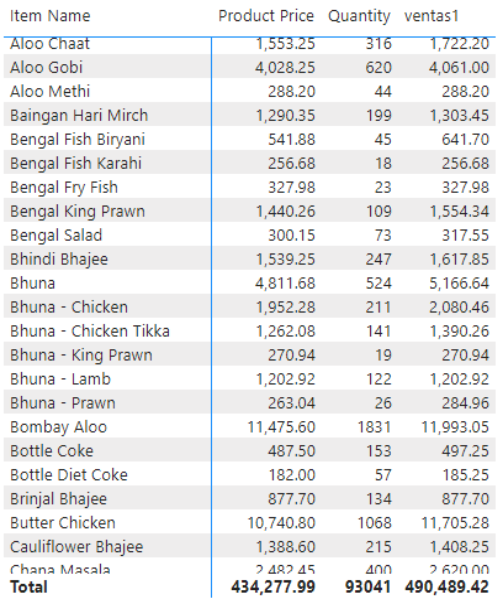
\includegraphics[scale=0.4]{images/1}
	\centering 
	\caption{0 es muerto; 1 es sobreviviente.}
\end{figure}
	\end{sol}
	\item Haga un modelo que pueda predecir la probabilidad de que los pasajeros sobrevivan.
	\begin{sol}
		content..
	\end{sol}
	\item Hay datos de pasajeros que no se tiene el “tag” si sobrevivieron o no. Corra el modelo para entender si los pasajeros sobrevivieron.
	\begin{sol}
		content..
	\end{sol}
\end{enumerate}

%---------------------------
%\bibliographystyle{apa}
%\bibliography{referencias.bib}

\end{document}